\twocolumn[\vspace*{-1.8ex}\section{ANNEX A:\endgraf FORMATTING OF AUTHORS AND AFFILIATIONS}\vspace*{\baselineskip}]

\flushcolsend

The names of authors, their organizations/affiliations
and postal addresses should be grouped by affiliation and
listed in \SI{12}{pt} upper- and lowercase letters. The name of
the submitting or primary author should be first, followed
by the coauthors, alphabetically by affiliation. If the
author list for a given affiliation spans multiple lines,
please be sure to break the line in a manner that does not
split the author’s initials from the author’s last name. This
is easily done by placing unbreakable spaces between the
initials and last name. The affiliation name and address
are also best kept together on the same (but not necessarily
separate) line, wherever possible. (See, for example,
the entry for GSI in the following). In cases where authors
have multiple affiliations, the secondary affiliation is
inserted below the author/primary affiliation listing and is
indicated with a superscript, as shown in the following.


Footnotes on the title and author lines may be used for
acknowledgements and e-mail addresses, using a non-numeric
sequence of characters (\textsuperscript{*}, \textsuperscript{†},
\textsuperscript{‡}, \textsuperscript{§}, \textsuperscript{\P}
as generated by \LaTeX's \verb|\footnote| command).

For examples of the preferred formatting of authors and
affiliations, please consult the following list of JACoW
collaboration members.

For manuscripts submitted by large collaborations with
potentially many tens of authors and where, additionally,
there may be page number limitations, a format consisting
of the principle author’s name and institute, followed by
“on behalf of the … collaboration”, is preferred.


\clearpage
%
% Include the title/author page of the JACoW Coolaboration
%
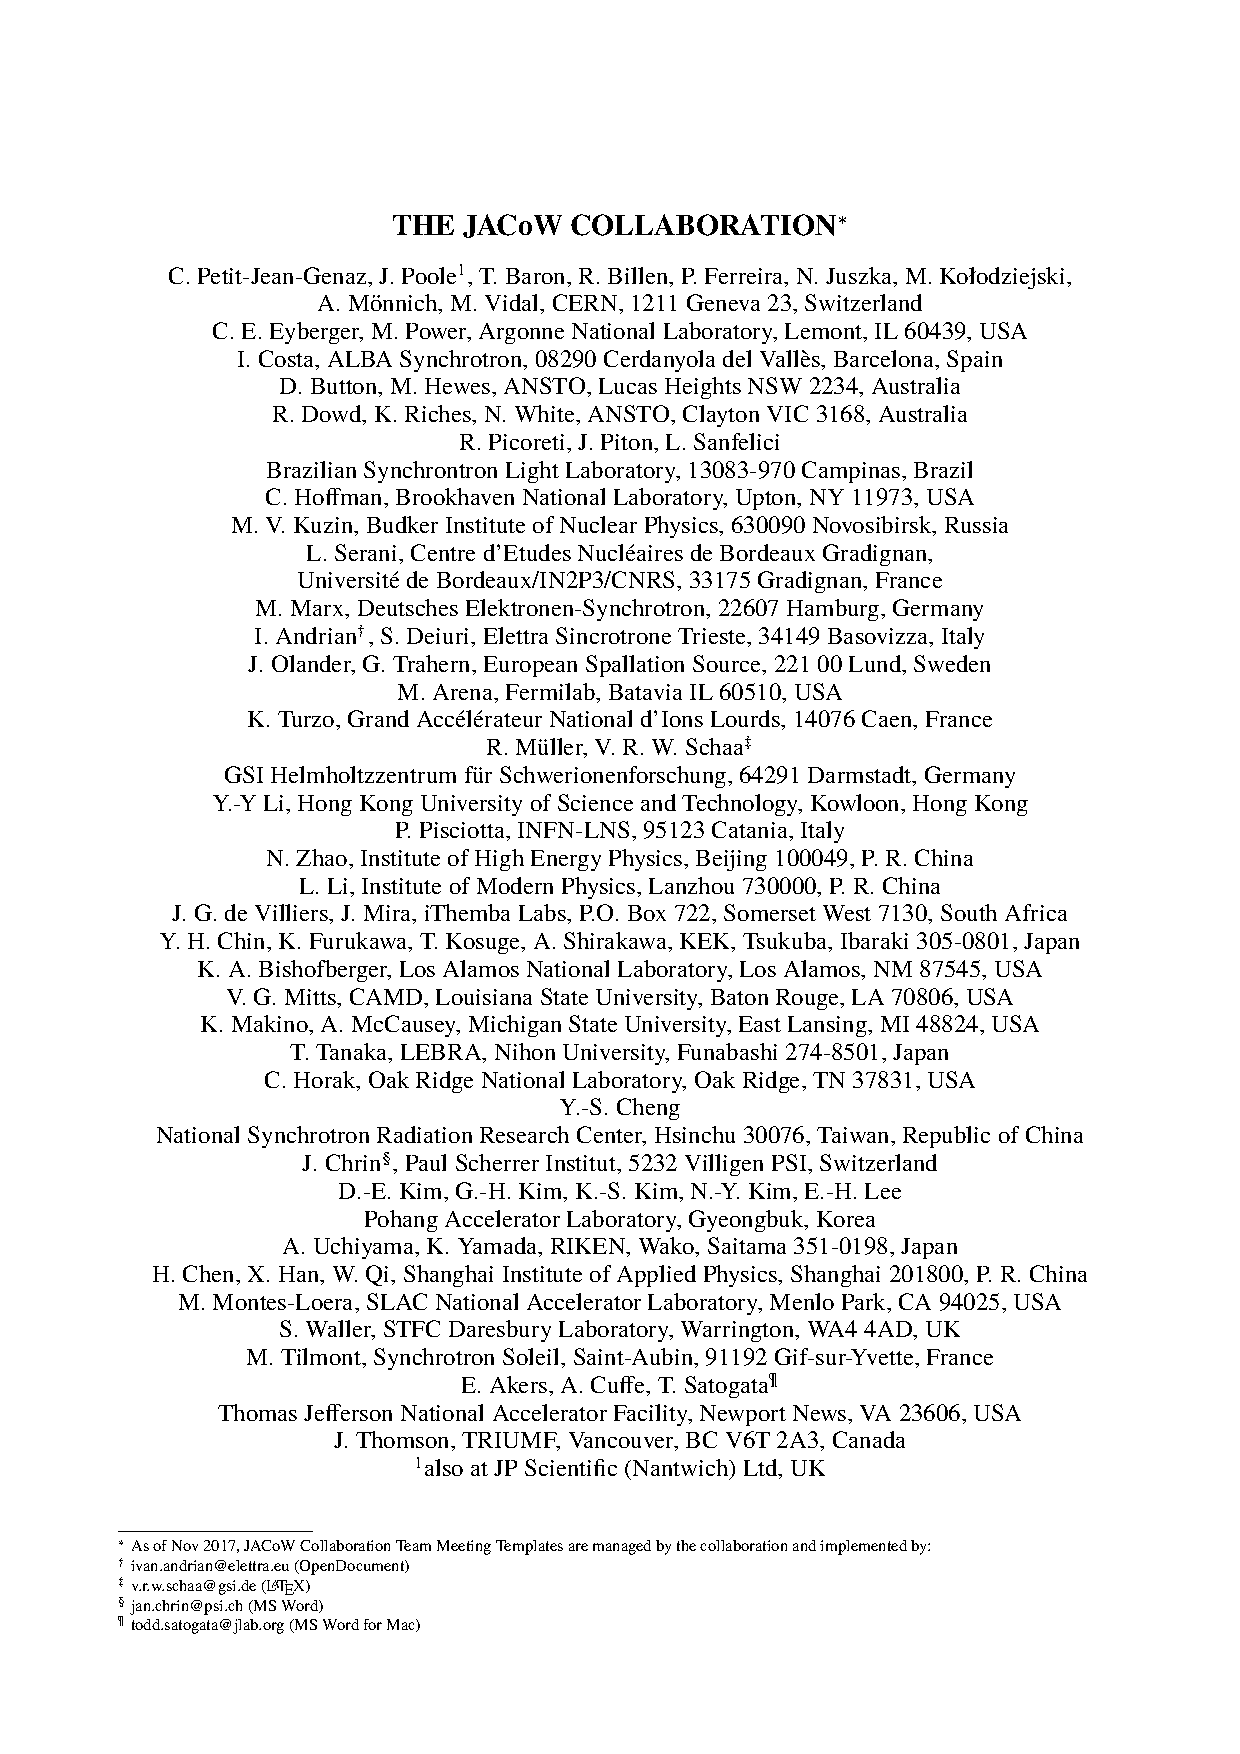
\includepdf[pages=-, noautoscale, pagecommand={}]{jacow-collaboration-2018.pdf}{}

\clearpage

\twocolumn[\vspace*{-1.8ex}\section{ANNEX B:\endgraf IEEE REFERENCE STYLE GUIDE AS APPLIED TO \NoCaseChange{JACoW} PAPERS, \break PERIODICALS AND OTHER WORKS}\vspace*{\baselineskip}]

\subsection{Referencing JACoW Proceedings}

The format for published JACoW proceedings papers is detailed in the following 
and can also be readily deduced from Refs. [1-3]. At the very minimum, sufficient 
information should be given to enable readers to clearly identify the paper and 
to facilitate its import into digital databases.
\vspace*{-.6\baselineskip}

\subsubsection{Author Listing} Careful attention should be given to the
placing of commas and the use of ‘and’ in the author list.
In particular, for the case of three or more authors
(as in [3]), a comma also follows the penultimate author.
The preference for ‘\emph{et al.}’\ takes precedence when the number
of authors becomes large (e.g., $>$6).
\vspace*{-.6\baselineskip}

\subsubsection{Paper Title} As is modern practice in references, the title
of the paper is written in sentence case, i.e., only the
initial letter of the first word in the title is capitalized.
Proper nouns, however, also have a capital. Capital letters
appearing in acronyms likewise remain unaltered
\vspace*{-.6\baselineskip}

\subsubsection{Conference Proceedings} The proceedings title is
written in title case in italics using standard abbreviations,
such as \emph{Int.} and \emph{Conf.} The preposition, ``in'', in normal
font, precedes the proceedings title. The location,
i.\,e., city, state (if USA), and country of the conference
venue, the month (three-letter abbreviation) and the year
the conference took place, is then listed. Finally, details
pertaining to the paper itself, such as the conference paper
ID, mandatory page numbers, and the digital object
identifier (DOI), if existing, are listed in the given order.
A monospace font for the DOI is used so as to help
distinguish it from normal text. In \LaTeX{}
the ‘url’ package is used. The conference
paper ID is optional and may be included in the absence
of a DOI to facilitate a search through internet search
engines. DOIs have been assigned to all JACoW
publications appearing in recent proceedings and will
likewise be assigned to articles from conferences further
past, in due course. The use of DOIs is strongly
emphasized.

The complete or abbreviated form for citations, as
shown in the following section, is advocated. The former
is more informative to readers outside the immediate
conference sphere, and will further serve to avoid
potential ambiguities in cases where an acronym is not
unique. Both forms, however, when adhered to, ensure a
proper import into digital libraries and information
sources such as INSPIRE, Scopus, and Google Scholar.
Authors are also reminded to make a distinction between
papers published in JACoW proceedings (which have
page numbers and, in the case of recent publications,
DOIs) and those papers that may have been presented at
past JACoW conferences but were not published~[4].
References to contributions presented at the same
conference should be written as shown in [5]; the wording
“this conference” may be optionally appended.

\subsection{Referencing Periodicals and Other Sources}

The IEEE style is also shown for periodicals [6-11],
online sources [12], books [13, 14], internal reports [15],
theses [16], manuals or handbooks [17], patents [18] and
unpublished material [19, 20]. Examples of correctly
formatted references can also be found at the JACoW website,
under ‘Formatting Citations’ which is reached through the
‘for Authors’ link.

\subsection{Alignment of References}

In the \LaTeX{} template, \verb|\bibliography{9}| is used for
when the total number of references is less than ten. This
should be changed to \verb|\bibliography{99}| if the number of
references is ten or more.

\patchcmd\thebibliography{\section*{REFERENCES\@mkboth {REFERENCES}{REFERENCES}}}{}{}{}
\section{PAPER PUBLISHED IN A CONFERENCE PROCEEDINGS}

\definecolor{jgreen}{cmyk}{0.81, 0.00, 0.97, 0.00}
\definecolor{jred}{cmyk}  {0.00, 0.99, 1.00, 0.00}
\definecolor{jgrepc}{cmyk}{0.74, 0.05, 1.00, 0.00}
\definecolor{jblue}{cmyk} {0.87, 0.54, 0.00, 0.00}
\definecolor{jvio}{cmyk}  {0.41, 0.82, 0.00, 0.00}
\definecolor{jbook}{cmyk} {0.28, 0.88, 0.79, 0.25}
\definecolor{jrept}{cmyk} {0.07, 0.70, 1.00, 0.00}
\definecolor{jmanu}{cmyk} {0.28, 0.77, 1.00, 0.23}
\definecolor{junpu}{cmyk} {0.00, 0.83, 0.65, 0.00}


\subsection{Complete Form}

\newcommand{\CCom}[2]{\newline\textcolor{#1}{[#2]}}
%\begin{thebibliography}{99}   % Use for  10-99  references
\begin{thebibliography}{9} % Use for 1-9 references
	
	\bibitem{item:1-1}
	A.~Alpha and B.~T.~Beta, “Novel techniques for future TeV electron accelerators”,
	in \textit{Proc. 8th Int. Particle Accelerator Conf. (IPAC’17)},
	Copenhagen, Denmark, May 2017, 
	pp. 567-569, \url{doi:10.18429/JACoW-IPAC2017-PAPERID}
	\CCom{jgreen}{Conference Proceedings, two authors; DOI encouraged}

	\bibitem{item:1-2}
	A.~Alpha \emph{et al.},
	“A new 12\,GHz electron linear accelerator”,
	in \emph{Proc. 28th Linear Accelerator Conf. (LINAC’16)},
	East Lansing, MI, USA, Sep. 2016, pp. 27-31, \newline
	\url{doi:10.18429/JACoW-LINAC2016-PAPERID}
	\CCom{jgreen}{Conference Proceedings, for six or more authors use \emph{et al.};	
		 DOI encouraged}
	
	\bibitem{item:1-3}	
	A.~Alpha, B.~T.~Beta, C.~Gamma, and D.~Delta,
	“An overview of control systems”,
	in \emph{Proc. 13th Int. Conf. on Accelerator and Large Experimental Physics Control Systems (ICALEPCS’11)}, Grenoble, France, Oct. 2011,
	paper TUP014, pp. 89--91.
	\CCom{jgreen}{Conference Proceedings, four authors; optional paper ID
	in the absence of a DOI}
\end{thebibliography}

\vspace*{-.5\baselineskip}
\subsection{Abbreviated Form}

\begin{thebibliography}{9} % Use for 1-9 references
	\bibitem{item:2-1}
	A.~Alpha and B.~T.~Beta, “Novel techniques for future TeV electron accelerators”,
	in \textit{Proc. IPAC’17}, Copenhagen, Denmark, May 2017, 
	pp. 567-569, \newline
	\url{doi:10.18429/JACoW-IPAC2017-PAPERID}
	\CCom{jgreen}{Conference Proceedings, two authors; DOI encouraged}
	
	\bibitem{item:2-2}
	A.~Alpha \emph{et al.},
	“A new 12\,GHz electron linear accelerator”,
	in \emph{Proc. LINAC’16},
	East Lansing, MI, USA, Sep. 2016, pp.\,27-31, 
	\url{doi:10.18429/JACoW-LINAC2016-PAPERID}
	\CCom{jgreen}{Conference Proceedings, for six or more authors use \emph{et al.};	
		 		  DOI encouraged}
	
	\bibitem{item:2-3}	
	A.~Alpha, B.~T.~Beta, C.~Gamma, and D.~Delta,
	“An overview of control systems”,
	in \emph{Proc. ICALEPCS’11}, Grenoble, France, Oct. 2011,
	paper TUP014, pp. 89--91.
	\CCom{jgreen}{Conference Proceedings, four authors; optional paper ID
				  in the absence of a DOI}
\end{thebibliography}

\section{UNPUBLISHED PAPER PRESENTED AT A PREVIOUS CONFERENCE}

\subsection{Complete Form}

\begin{thebibliography}{9} % Use for 1-9 references
\setcounter{enumi}{3}
 \bibitem{item:41}
	A.~Alpha and B.~T.~Beta,
	“An interesting talk but paper not submitted”,
	presented at the 5th Int. Particle Accelerator Conf. (IPAC’14),
	Dresden, Germany, Jun. 2014, paper MOAX01, unpublished.
	\CCom{jred}{Unpublished paper; conference name in normal font; paper
	ID may only be given if material supplementing the proceedings
	exists on the JACoW website, e.\,g., PDF of talk}
\end{thebibliography}

\subsection{Abbreviated Form}

\begin{thebibliography}{9} % Use for 1-9 references
\setcounter{enumi}{3}
 \bibitem{item:42}
	A.~Alpha and B.~T.~Beta,
	“An interesting talk but paper not submitted”,
	presented at IPAC’14,
	Dresden, Germany, Jun. 2014, paper MOAX01, unpublished.
	\CCom{jred}{Unpublished paper; conference name in normal font; paper
	ID may only be given if material supplementing the proceedings
	exists on the JACoW website, e.\,g., PDF of talk}
\end{thebibliography}


\section{PAPER PRESENTED AT THE CURRENT CONFERENCE}

\subsection{Complete Form}

\begin{thebibliography}{9} % Use for 1-9 references
\setcounter{enumi}{4}
 \bibitem{item:51}
	A.~Alpha and B.~T.~Beta,
	“An interesting talk at this conference”,
	presented at the 9th Int. Particle Accelerator
	Conf. (IPAC’18), Vancouver, Canada, Apr.-May 2018, 
	paper MOAB01, this conference.
	\CCom{jgrepc}{Current conference; conference name in normal font; 
				  the wording “this conference” is optional}
\end{thebibliography}

\subsection{Abbreviated Form}

\begin{thebibliography}{9} % Use for 1-9 references
\setcounter{enumi}{4}
	\bibitem{item:52}
	“An interesting talk at this conference”,
	presented at IPAC’18, Vancouver, Canada, Apr.-May 2018, 
	paper MOAB01, this conference.
	\CCom{jgrepc}{Current conference; conference name in normal font; 
				  the wording “this conference” is optional}
\end{thebibliography}


\vspace*{-.5\baselineskip}
\section{PAPER PUBLISHED IN, OR SUBMITTED TO, A PERIODICAL}

\begin{thebibliography}{99} % Use for 1-9 references
  \setcounter{enumi}{5}
	\bibitem{item:6}
		P.~Mercury \emph{et al.},
		“Title of paper published in journal”,
		\emph{Phy.~Rev.~	Lett.}, vol. 114, no. 5,
		p. 050511, Feb. 2014,
		\url{doi:10.1103/PhysRevLett.114.050511}
	\CCom{jblue}{Periodical, Phys. Rev. Lett.;
		             issue no. and month may be omitted}

	\bibitem{item:7}
		P.~Venus \emph{et al.},
		“New techniques in laser wakefield accelerators”,
		\emph{Phys. Rev. ST Accel. Beams}, vol. 18,
		p. 120198, Dec.~2015, \newline
		\url{doi:10.1103/PhysRevAccelBeams.18.120198} 
	\CCom{jblue}{Periodical, Phys. Rev. ST Accel. Beams;
			              month may be omitted}

	\bibitem{item:8}
		T.~Earth \emph{et al.},
		“Low dose irradiation impact on modern silicon detectors”,
		\emph{Nucl. Instr. Meth.}, vol. 692, pp. 256--280, 2014,
		\url{doi:10.1016/j.nima.2014.11.022}
	\CCom{jblue}{Periodical, Nucl. Instr. Method.}
	
	\bibitem{item:9}
		T.~Earth, L.~Moon, and A.~Belt,
		“Temporal correlations of x-ray free electron lasers”,
		\emph{Optics Express}, vol. 20, pp. 11396--11404, 2012,
		\url{doi:10.1364/OE.20.11396}
	\CCom{jblue}{Periodical, Optics Express}

	\bibitem{item:10}
		J.~B.~Good,
		“A paper accepted for publication”,
		\emph{Phys. Rev. Lett.}, to be published.
	\CCom{jblue}{Periodical, paper accepted for publication
		              by Phys. Rev. Lett.}

	\bibitem{item:11}
		G.~D.~Read,
		“Title of paper submitted for publication”,
		submitted for publication.
	\CCom{jblue}{Paper submitted for publication; the name of the
					  periodical does not appear}
\end{thebibliography}

\vspace*{-.5\baselineskip}
\section{ONLINE SOURCE}

\begin{thebibliography}{99} % Use for 1-9 references
  \setcounter{enumi}{11}
	\bibitem{item:121}
		JACoW, \url{http://www.jacow.org} 
		\CCom{jvio}{online source; no hyperlink, no period at end of URL unless there is a
					trailing “/” as shown below. A monospace font should be used, this is
					achieved using the ‘url’ package in \LaTeX}

  \setcounter{enumi}{11}
	\bibitem{item:122}
		JACoW, \url{http://www.jacow.org/}.  
		\CCom{jvio}{online source; no hyperlink, period after traling “/” in
					URL allowed. A monospace font should be used, this is
					achieved using the ‘url’ package in \LaTeX}

\end{thebibliography}

\section{CITATIONS TO BOOKS}

\begin{thebibliography}{99} % Use for 1-9 references
	\setcounter{enumi}{12}
	\bibitem{item:13}
		T.~Earth and L.~Moon,
		“Title of chapter in the book”,
		in \emph{Title of Book}, R Mars, Ed. New York, NY, USA:
		Wiley, 1994, pp.~42--48. 
	\CCom{jbook}{Chapter in book}
	
	\bibitem{item:14}
		A.~Belt, \emph{Title of Book}. Cambridge, MA, USA:
		MIT Press, 1986. 
	\CCom{jbook}{Book}
\end{thebibliography}

\section{REPORTS AND THESES}

\begin{thebibliography}{99} % Use for 1-9 references
	\setcounter{enumi}{14}
	\bibitem{item:15}
		G. Jupiter \emph{et al.},
		“Title of report”, CERN, Geneva, Switzerland,
		Rep. CERN-2012-333, Oct. 2012.
	\CCom{jrept}{Report}

	\bibitem{item:16}
		A.~Student, “Title of thesis”,
		Ph.D. thesis, Phys. Dept.,
		Karlsruher Institut für Technologie, Karlsruhe,
		Germany, 2014.
	\CCom{jrept}{Thesis}
\end{thebibliography}

\section{MANUAL}

\begin{thebibliography}{99} % Use for 1-9 references
	\setcounter{enumi}{16}
	\bibitem{item:17}
		\emph{IEEE Editorial Style Manual},
		IEEE Periodicals,
		Piscataway, NJ, USA, Oct. 2014, pp. 34-52;
		\url{http://www.ieee.org/documents/style_manual.pdf} 
	\CCom{jmanu}{Handbook/Manual, no hyperlink, no period after URL}
\end{thebibliography}

\section{PATENTS}

\begin{thebibliography}{99} % Use for 1-9 references
	\setcounter{enumi}{17}
		\bibitem{item:18}
		A.~N.~Inventor,
		“Title of patent”,
		Patent Authority and No., Jan. 20, 2016.

\end{thebibliography}

\section{UNPUBLISHED WORK AND PRIVATE COMMUNICATION}

\begin{thebibliography}{99} % Use for 1-9 references
	\setcounter{enumi}{18}
	\bibitem{item:19}
		P.~Neptune, “Title of paper”, unpublished.
	\CCom{junpu}{Unpublished}
	
	\bibitem{item:20}
	P.~Uranus, private communication, Jun. 2015.
	\CCom{junpu}{Private communication}

\end{thebibliography}

\newpage

\twocolumn[\vspace*{-1.8ex}\section{ANNEX C:\endgraf THE DILIGENT AUTHOR’S CHECKLIST}\vspace*{\baselineskip}]
\flushcolsend

\subsection{Common Oversights}

In order to lessen the load on a small team of editors
and to help expedite publication of the Proceedings, authors
are kindly asked to give themselves an extra few
minutes to go over the following points, which highlight
the most common errors, before uploading their paper. By
providing a properly formatted JACoW paper, the Proceedings
Office is able to benefit from an autodistill process
which automatically converts the author's PDF file
into a version that adheres to the JACoW-compliant PDF
standard. The process further ensures that all fonts required
to view the entire document are embedded, rendering
a final PDF that qualifies technically for publication.


\subsection{Author and Affiliation Listing}

The names of authors and their affiliations should be in
\SI{12}{pt} uppercase and lowercase letters, with standard,
roman fonts (i.\,e., not italics). When there is more than
one author, the submitting author should be first, followed
by the coauthor. Coauthors should be grouped by affiliation
and then be listed alphabetically. Please refer to \textbf{ANNEX~A}
for further details and examples, particularly for
the case where authors have multiple institutes.

\subsection{SPMS Database and Final Manuscript Validation}

Primary authors are reminded that it is their
responsibility to verify the accuracy of the title, abstract,
and coauthor/institute listing, and that these are identical
in both the final manuscript and SPMS database. This is
required to ensure the proper indexing of author/coauthor(s) 
appear in the published proceedings.

\subsection{Subsection Headings}

Subsection Headings are in \SI{12}{pt} \emph{italic} lowercase and uppercase.
The initial letter of every principle word is capitalized,
and the heading is left aligned in the column.

\subsection{Figure Captions}

Figure captions should be placed \emph{below} the figure and
centred if on one line, but justified if spanning two or
more lines:
\begin{center}
	Figure 1: A one line figure caption is centred.
\end{center}
\begin{justify}
	Figure 2: A lengthy figure caption that spans
	two lines is justified.
\end{justify}
Note the colon “:” after the figure number and the period
“.” at the end of the caption.


When referring to a figure from within the text, the
convention is to use the abbreviated form, i.\,e., Fig.~1,
\emph{unless} the reference to the figure is at the start of the sentence:
\begin{quote}
	Figure 1 shows a schematic view of...
	
	... as shown in Fig.~1.
\end{quote}

\subsection{Table Headings}

Table captions should be placed \emph{above} the table and
centred if on one line, but justified if spanning two or
more lines:
\begin{center}
	Table 1: Table Heading
\end{center}
\begin{justify}
	Table 2: A Particularly Long Table Heading
	Spanning Two Lines
\end{justify}

Note the colon ":" after the table number, that the initial
letters of the principle words in the table heading are
capitalized, and the absence of a period at the end of the
caption.

When referring to a table from within the text, the convention
is \emph{not} to abbreviate, i.\,e., Table 1.

\subsection{Equations}

If a displayed equation requires a number, it should be
placed flush with the right margin of the column. 

\subsection{Units}

An unbreakable space should always precede a unit. In \LaTeX{} use
a “\verb|\,|” or the ‘siunitx’ package to format units.
Examples are:
\SI{3}{keV}, \SI{4}{GeV}, \SI{100}{kW}, \SI{7}{µm}.

\subsection{References}

References are written in \SI{9}{pt} size and should be neatly
presented in a consistent format with reference numbers
aligned. Please refer to \textbf{ANNEX~B} for the preferred format
and proper alignment.

Please also ensure that references in the text are cited in
sequential order.

\flushend
